%Om filen typsätts som del av hela rapporten så finns \master definierat i början och ingen \begin{document} och \end{document} får finnas, men för att kunna typsätta filen för sig är dem ett måste! \newcommand{\master}{} krävs i början på huvudrapporten!

\ifdefined\master
\else
	\documentclass[twocolumn]{article}
\usepackage{graphicx}
\usepackage{float} %gör så att man kan placera bilder exakt mha [H]
	%\input{../preamble}
	\begin{document}
\fi
%text goes here!
\section{Lab demonstration}
To demonstrate the functionality of the program an easy lab-assignment was performed. A RC-circuit was connected like figure \ref{fig:RCcircuit}, the circuit is a low-pass filter with the cutoff frequency at $f=1.5~kHz$. 
	\begin{figure}[h]
	\centering
		\fbox{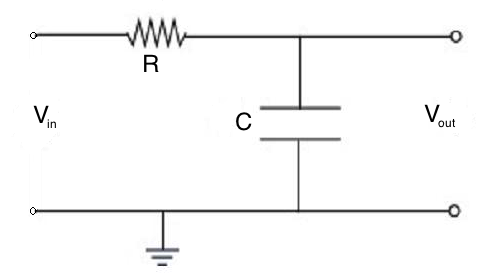
\includegraphics[width=4cm]{Figure/rc-circuit}}
		\caption{RC-circuit}
		\label{fig:RCcircuit}
	\end{figure}

Start with connecting the oscilloscope, multimeter, function- and voltage generator to the computer using the GIPB-port. Check that every device has a different GPIB-address to be sure that all will work.  

\subsection{Assignment 1}
The first assignment is about looking at the difference between the in- and out-signal. Set the function generator frequency to $1~kHz$ and the amplitude to $3~V$. Also add the GIPB-address of the function generator and the oscilloscope. Click \emph{Set} at the bottom of the function generator panel and select \emph{oscilloscope picture} in the popup-menu at the out panel. Next, add the GPIB-address to the oscilloscope and click start to get a picture from the oscilloscope. Figure \ref{oscilloskopPicture} shows a picture from the oscilloscope with the settings mentioned above. 
	\begin{figure}[H]
	\centering
		\fbox{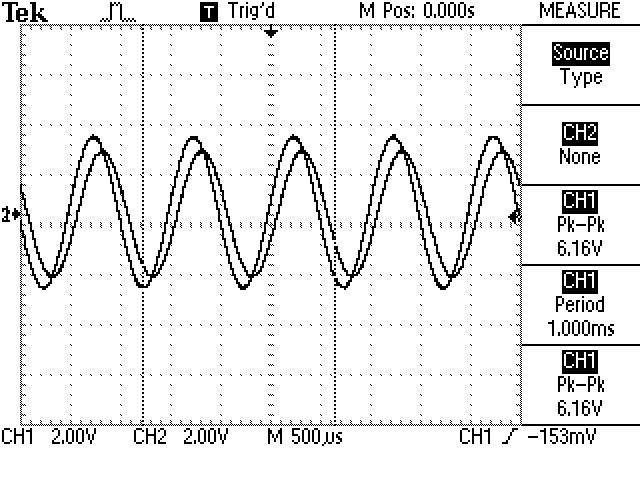
\includegraphics[width=6cm]{Figure/screenshot.png}}
		\caption{Oscilloscope picture.}
		\label{oscilloskopPicture}
	\end{figure}

Now use the export function to put the figure in a report by selecting the \emph{LaTeX} alternate in export popup-menu. It will be possible to change the title and figure labels by typing the wanted label name in the \emph{X-Label} and \emph{Y-Label} text boxes. The figure title is changed by typing in the \emph{Title} text box. The LaTeX figure caption and reference label can be set by typing in the \emph{Label} and \emph{Caption} text boxes. Finally, type a figure name and click \emph{export} and chose a location for the files to be saved.

\subsection{Assignment 2}
Connect the multimeter to measure the voltage over the resistor. Change the output panel to multimeter, select the \emph{Voltage [AC]} in the measuring popup-menu, add the GPIB-address for the multimeter and press start button. The multimeter will be displayed in the black text box in the output panel. By clicking the \emph{Stop}-button multimeter will stop and the data can be saved to a .mat file or present in a stem-graph by exporting the figure. The generated stem-graph is presented in Figure \ref{stem}.
	\begin{figure}[H]
	\centering
		\fbox{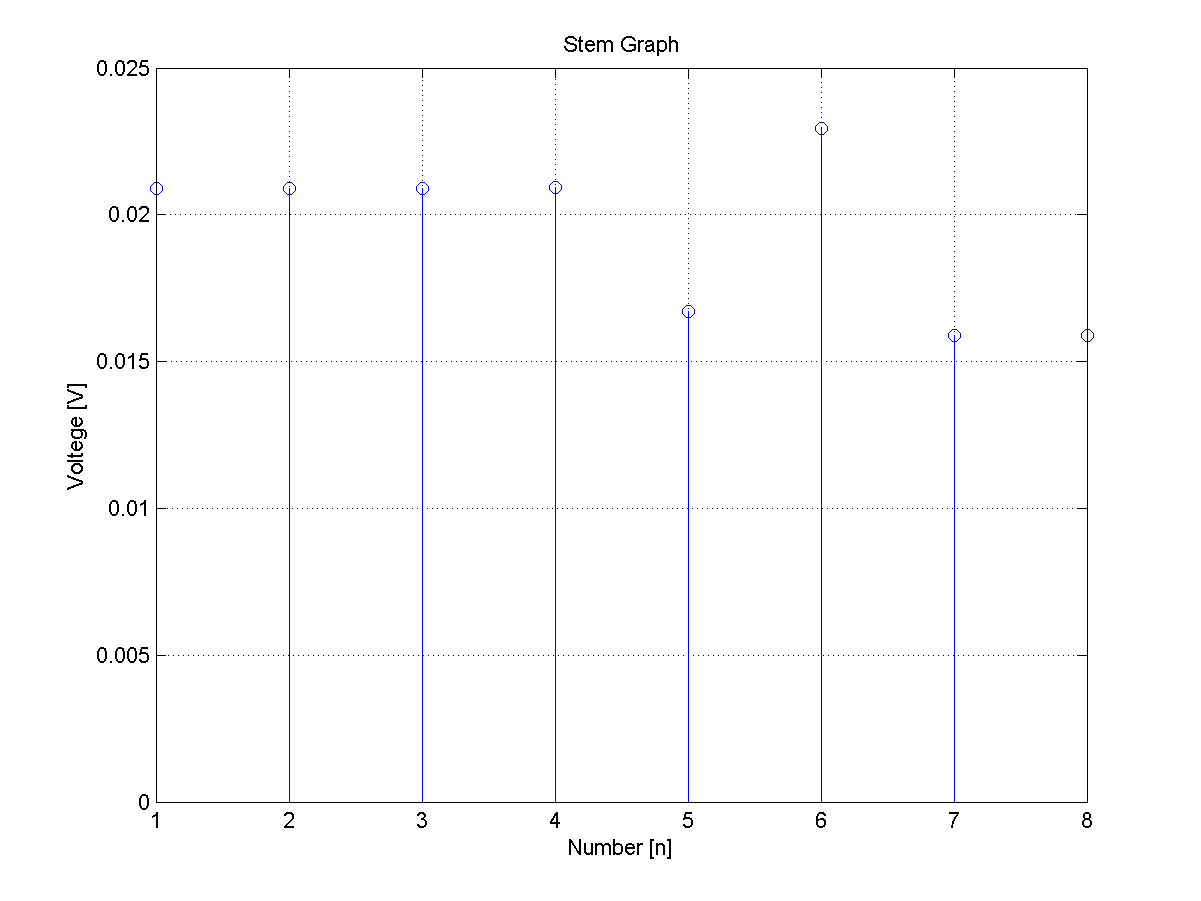
\includegraphics[width=6cm]{Figure/stem.png}}
		\caption{Stem graph from multimeter measurment}
		\label{stem}
	\end{figure}

\subsection{Assignment 3}
Move the multimeter probes to measure the output voltage and change to \emph{frequency sweep} in the input popup-menu and set the start- and end frequency to $0~Hz$ and $3000~Hz$ and the step length to $100~Hz$ use \emph{Sine} as waveform with an amplitude $3~V$ and click \emph{Start sweep}. This will take some time.\\
\\
The generated bode graph figure \ref{bode} can be exported to a Word-document in the same way as the LaTeX export, the generated frequency and voltage can also be saved for other use in Matlabs workspace. 
	\begin{figure}[H]
	\centering
		\fbox{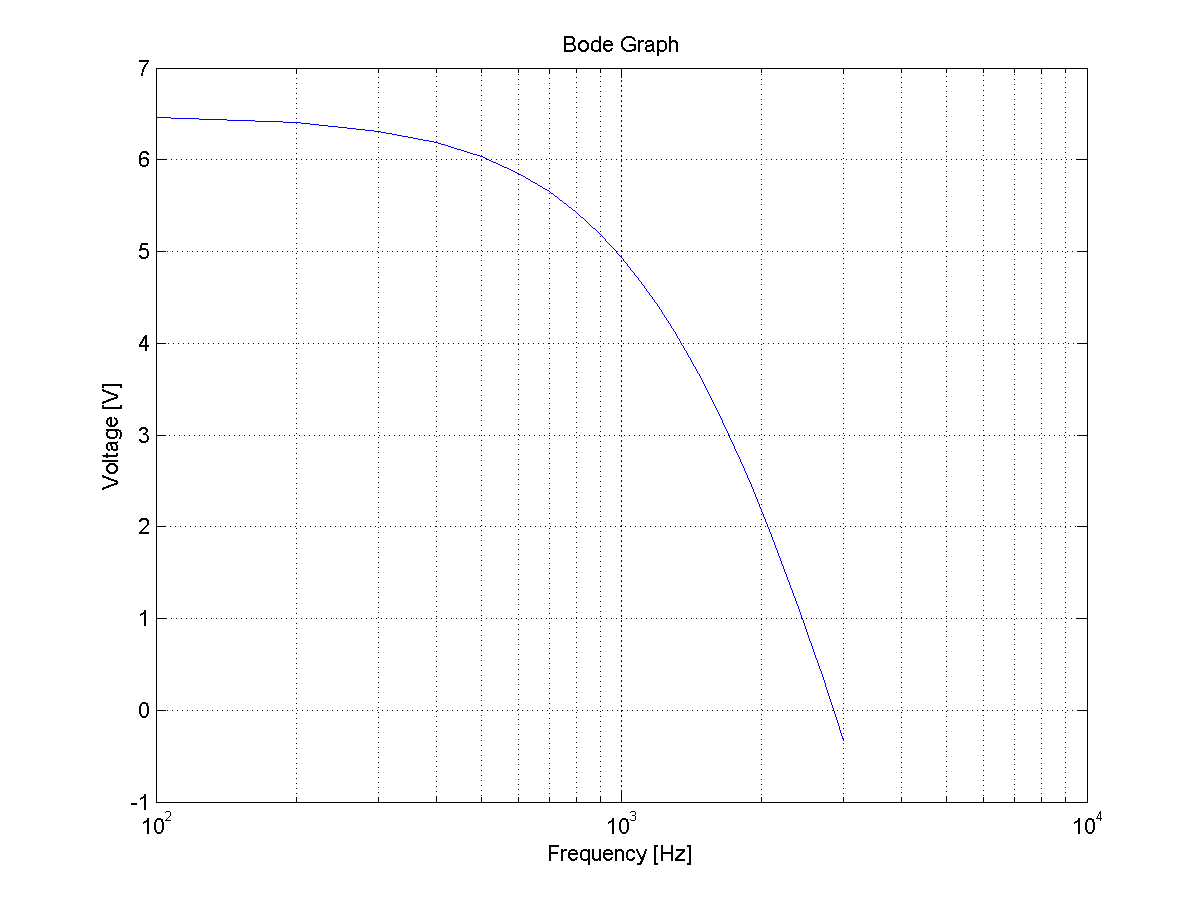
\includegraphics[width=6cm]{Figure/bode.png}}
		\caption{Bode graph}
		\label{bode}
	\end{figure}   

\ifdefined\master
\else
	\end{document}
\fi